\documentclass[12pt]{article}
\usepackage{sbc-template}
\usepackage[utf8]{inputenc}
\usepackage{listings}
\usepackage{xcolor}
\usepackage[english]{babel}
\usepackage{graphicx}

\lstdefinelanguage{JavaScript}{
  keywords={break, case, catch, continue, debugger, default, delete, do, else, finally, for, function, if, in, instanceof, new, return, switch, this, throw, try, typeof, var, void, while, with, let, const},
  morecomment=[l]{//},
  morecomment=[s]{/*}{*/},
  morestring=[b]',
  morestring=[b]",
  ndkeywords={class, export, boolean, throw, implements, import, this, extends, super},
  sensitive=true
}

\lstset{
  language=JavaScript,
  basicstyle=\ttfamily\small,
  keywordstyle=\color{blue},
  ndkeywordstyle=\color{orange},
  commentstyle=\color{gray},
  stringstyle=\color{green},
  breaklines=true,
  frame=single,
  captionpos=b,
  numbers=left,
  numberstyle=\tiny\color{gray},
  stepnumber=1,
  numbersep=5pt,
  showstringspaces=false,
  tabsize=2,
  backgroundcolor=\color{white},
  showspaces=false,
  showtabs=false,
  caption={Exemplo de código JavaScript},
  label={lst:exemplo-js}
}


\title{Using Generative AI on-premise in code review process}
\author{Pedro A. D. Kfuri\inst{1}, Advisor: Humberto Torres Marques Neto\inst{1} }
\address{
Instituto de Ciências Exatas e Informática \\
Pontifícia Universidade Católica de Minas Gerais (PUC MG)
  \email{pedrokfuri@outlook.com, humberto@pucminas.br}
}

\begin{document} 
\maketitle
\begin{abstract}
This study explores the integration of Generative AI to automate code reviews in GitLab and Github merge requests using Ollama, an on-premise AI inference engine. A webhook connects to GitLab's or Github's API, automatically analyzing code changes, providing structured feedback, and helping to decide on request approval or rejection. This solution improves review efficiency, reduces waiting times, and maintains data privacy by operating on local infrastructure. The proposed approach contributes to AI-assisted software engineering by streamlining code quality assurance in collaborative development environments.
\end{abstract}

\section{Introduction}
The code review process is a critical yet time-consuming step in software development, often causing delays in merge request approvals due to human availability constraints. As teams grow and repositories scale, the inefficiencies of manual reviews become increasingly evident, leading to bottlenecks that hinder continuous integration and deployment. Recent advancements in Generative AI offer a promising solution by enabling automated code analysis and review. This study proposes an on-premise integration of Generative AI into GitLab\footnote{https://gitlab.com} and Github\footnote{https://github.com} workflows using Ollama\footnote{https://ollama.com}, a locally deployed AI inference engine.
    
By implementing a webhook that connects to GitLab’s and Github's API, the system analyzes merge requests, provides feedback on code quality, and determines approval or rejection based on predefined criteria. This approach ensures enhanced review consistency, reduced lead time, and adherence to best coding practices without relying on external AI services, preserving data privacy. The research contributes to the field of AI-assisted software engineering by evaluating the efficiency and accuracy of automated code review in real-world development environments.

\section{Background}

Artificial Intelligence (AI) and Machine Learning (ML) have significantly transformed DevOps, particularly in automating processes within Continuous Integration/Continuous Deployment (CI/CD) pipelines. AI-driven automation enhances efficiency, reduces manual effort, and improves software quality. Among the most promising advancements is the use of Large Language Models (LLMs) for automated code review, which provides real-time feedback, ensures coding standard adherence, and identifies potential security vulnerabilities. Faster feedback loops further streamline development cycles, contributing to higher productivity. \cite{AIDrivenDevops}

AI-enhanced DevOps, often referred to as "Intelligent DevOps," integrates predictive analytics, anomaly detection, and self-healing mechanisms into software development workflows. Studies highlight that organizations leveraging AI in DevOps experience substantial reductions in time-to-market and operational costs. AI-driven monitoring and diagnostics improve system reliability, allowing developers to focus on strategic tasks rather than repetitive debugging and error detection. \cite{interdisciplinaryAIMLDevopsAutomation}
    
\subsection{Code Review}
Code review, the practice of systematically evaluating peers' code to enhance quality, works as a mechanism for quality assurance and a platform for collaborative learning. By scrutinizing code changes, reviewers disseminate domain-specific knowledge, coding standards, and architectural insights, thereby reducing siloed expertise and enhancing long-term maintainability. This knowledge transfer is vital in both open-source and industrial contexts, where onboarding new contributors and maintaining coherent codebases are ongoing challenges. For instance, in large tech organizations, code review is integral to sustaining code health across millions of lines of code. \cite{codereviewStudy}

The automation of code review tasks has emerged as a key research frontier, addressing scalability and efficiency concerns. Techniques such as reviewer recommendation, automated comment generation, and predictive models for change approval aim to streamline processes while preserving review efficacy. Deep learning models, pre-trained on vast corpora of code and natural language, now simulate human-like feedback, though challenges like dataset noise and metric reliability persist. \cite{codereviewStudy}

While LLMs enhance technical efficiency in code reviews, their inability to engage in the reciprocal social dynamics of accountability such as mutual justification, reputation building, and collective norm reinforcement, risks eroding the socio-technical fabric of software development. A critical insight is the potential for adaptive hybrid workflows: LLMs could serve as first-line technical validators, automating routine checks, while reserving nuanced, context-sensitive decisions  to human reviewers. \cite{accountability}

\subsection{CICD/DevOps Integration}
Continuous Integration and Continuous Delivery (CI/CD) constitute a foundational framework within modern software development practices, designed to streamline the integration, testing, and deployment of code changes. In this paradigm, developers frequently merge their contributions into a shared repository, triggering automated workflows that compile the codebase, execute test suites, and validate functionality. Successful iterations progress to deployment phases, ensuring rapid, reliable delivery of software updates while minimizing disruptions. \cite{AIDrivenDevops}

Code review represents a critical phase in the CI/CD pipeline, serving as a gatekeeping mechanism prior to code integration. Traditionally, this stage relies on human reviewers to assess code for errors, adherence to coding standards, and potential security vulnerabilities. \cite{aiDrivenAgile}

\subsection{Gitlab/Github API}
GitLab and GitHub provide REST APIs to programmatically access diff contents, which are structured representations of code changes between commits, branches, or merge/pull requests. The APIs return JSON formatted data detailing modified files, including metadata and line-level additions/deletions.


\lstset{basicstyle=\ttfamily, frame=single, language=JavaScript}
\begin{lstlisting}[caption={Github Patches API Endpoint}, label={lst:github-patches}]
GET /pulls/{pull_number}/files
\end{lstlisting}

\lstset{basicstyle=\ttfamily, frame=single, language=JavaScript}
\begin{lstlisting}[caption={Gitlab Diffs API Endpoint}, label={lst:gitlab-diffs}]
GET /{id}/merge_requests/{iid}/changes
\end{lstlisting}

GitHub’s Pull Request API outputs a files array with patch strings encoding line changes, while GitLab’s Merge Request API organizes diffs into a changes array with diff fields. Key distinctions include GitHub’s granular file statuses (e.g., added, modified) and GitLab’s emphasis on commit-level change aggregation. Both enable automated analysis of code modifications but differ in data structuring and endpoint granularity, reflecting platform-specific workflows.

\subsection{Generative AI}
Generative AI has emerged as a transformative tool in CI/CD processes, particularly for automating code generation, test case synthesis, and deployment script optimization. AI-driven tools like DeepCode and Codacy employ machine learning to analyze codebases and suggest improvements. While not explicitly labeled as "generative," these tools align with generative AI principles by predicting and generating code fixes, enforcing standards, and identifying vulnerabilities through pattern recognition. Generative models could further enhance such workflows by autonomously drafting code snippets, generating test scenarios, or refining deployment strategies based on historical data. \cite{AIDrivenDevops}

\subsection{Related Work}
Recent advancements in Large Language Models (LLMs), such as GPT-4 and BERT, have introduced novel opportunities to enhance DevOps workflows through intelligent automation and natural language processing. One key application is automated code analysis and generation, where LLMs streamline code reviews and suggest optimizations. For instance, GitHub Copilot assists developers by generating context-aware code snippets, reducing manual effort and accelerating development cycles. Similarly, tools like DeepCode and Codacy leverage LLMs to detect vulnerabilities, enforce coding standards, and propose fixes by analyzing historical codebases. These models improve code quality while integrating seamlessly into CI/CD pipelines, enabling real-time feedback during continuous integration. \cite{aiStreamlinedCICD}

Opportunities to research lie in the area of federated learning for training LLMs on decentralized DevOps datasets to preserve privacy, alongside developing multimodal LLMs capable of unified interpretation of code, logs, and user queries. Further exploration includes autonomous systems that dynamically optimize deployment pipelines through predictive resource allocation and adaptive rollback strategies. \cite{aiStreamlinedCICD}

\section{Methodology}
This implementation adopts a systematic approach that integrates artificial intelligence with DevOps practices to develop a scalable and robust application. The methodology is organized into distinct phases, each addressing specific aspects of the system’s nature: requirements analysis, system design, implementation and testing. For the LLM context there are two topics, which are model analysis and choice and Ollama instance deployment. The tests cover the integration between the webhook and code analysis tools' APIs and between the webhook and Ollama API.

\subsection{Requirements Analysis}
This section outlines the functional (RFxx) and non-functional (RNFxx) requirements of the system. Table~\ref{tab:requirements} summarizes these requirements.

\begin{table}[h!]
\centering
\begin{tabular}{|c|p{10cm}|}
\hline
\textbf{Requirement ID} & \textbf{Requirement Description} \\ \hline
RF01 & The application shall include an HTTP server to receive webhook requests via a REST API. \\ \hline
RF02 & The application shall allow configuration of the integration strategy via an environment variable, supporting the options “gitlab” or “github”. \\ \hline
RF03 & The application shall retrieve diff content from merge or pull requests by querying the API of the selected tool (GitLab or GitHub). \\ \hline
RF04 & The application shall interact with the local Ollama instance by sending diff content and receiving corresponding code analysis via its REST API. \\ \hline
RF05 & The application shall post a comment on merge or pull requests containing the code analysis provided by Ollama. \\ \hline
RNF01 & The Ollama instance must be properly configured and accessible over the internal network via a REST API. \\ \hline
RNF02 & The application must maintain reliable connectivity with the internal network. \\ \hline
RNF03 & The application must ensure consistent and reliable access to the GitLab API. \\ \hline
RNF04 & The application must ensure consistent and reliable access to the GitHub API. \\ \hline
RNF05 & The application shall incorporate a robust logging mechanism to record events and diagnostic information. \\ \hline
\end{tabular}
\caption{System Requirements}
\label{tab:requirements}
\end{table}

\subsubsection{Webhook}
A webhook is a method of augmenting or altering the behavior of a web application with custom callbacks. These callbacks are triggered by specific events, facilitating real-time data transmission between interconnected systems via HTTP requests. Unlike traditional polling mechanisms, where one system must repeatedly check another for updates, webhooks enable immediate notifications upon the occurrence of predefined events, thereby enhancing efficiency and responsiveness.

\subsubsection{Ollama}
Ollama is an open-source platform that enables users to run large language models (LLMs) locally on their machines. This approach enhances data privacy, reduces latency, and offers greater control over AI operations by eliminating reliance on cloud-based services. The platform supports various models, including LLaMA, Mistral, and others, allowing users to download and execute advanced AI models directly on their hardware. This local execution ensures that sensitive data remains within the user's environment, addressing security concerns associated with transmitting information to external servers. Ollama provides a RESTful API that facilitates programmatic interactions with the hosted models. Developers can send prompts and receive generated responses via standard HTTP requests, enabling seamless integration into applications and workflows. \cite{ollama}

While Ollama offers significant benefits, it also requires substantial computational resources. Running LLMs locally can be resource-intensive, necessitating considerable memory and processing power.

\subsection{Models}
Below is an overview of selected models compatible with Ollama, highlighting their characteristics, advantages, and potential drawbacks.

\subsubsection{Llama3.2:1b}
The Llama 3.2:1B model is a 1-billion-parameter multilingual LLM optimized for dialogue-based applications, including tasks like personal information management and multilingual knowledge retrieval. Its relatively small size allows for efficient operation on devices with limited computational resources. However, the reduced parameter count may impact performance on complex tasks requiring deeper contextual understanding. \cite{ollama}

\subsubsection{Llama3.2:3b}
With 3 billion parameters, the Llama 3.2:3B model offers enhanced performance over its 1B counterpart, excelling in instruction following, summarization, and prompt rewriting tasks. While it delivers improved accuracy and versatility, it demands more substantial computational resources, which may pose challenges for deployment on less powerful hardware. \cite{ollama}

\subsubsection{Codellama}
Code Llama is a specialized 7-billion-parameter model designed for programming-related tasks, including code generation, completion, and understanding. Its focus on code-related applications makes it a valuable tool for developers seeking AI assistance in software development. However, its large size necessitates significant memory and processing power, potentially limiting its usability on resource-constrained systems. \cite{codellama}

\subsubsection{DeepSeek-r1}
DeepSeek-R1 is a 7-billion-parameter model known for its robust performance across various language tasks. It serves as a viable alternative to other LLMs, offering competitive capabilities in text generation and comprehension. Nevertheless, similar to other large models, it requires ample computational resources for optimal operation, which may restrict its deployment in environments with limited hardware capabilities. \cite{deepseek}

\subsection{System Design}
\begin{figure}[htbp]
    \centering
    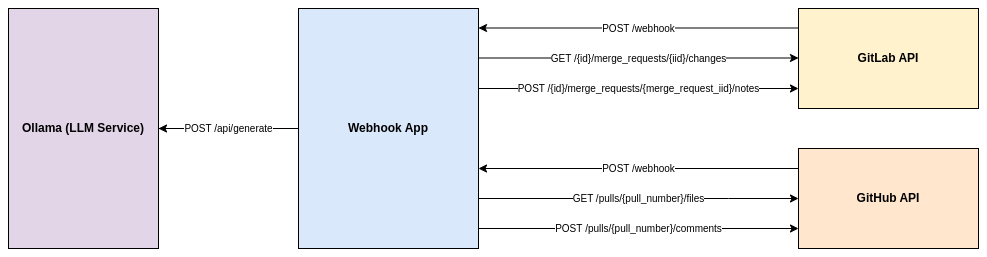
\includegraphics[width=1\textwidth]{systemdesign.png}
    \caption{System Design}
    \label{fig:systemdesign}
\end{figure}

\begin{figure}[htbp]
    \centering
    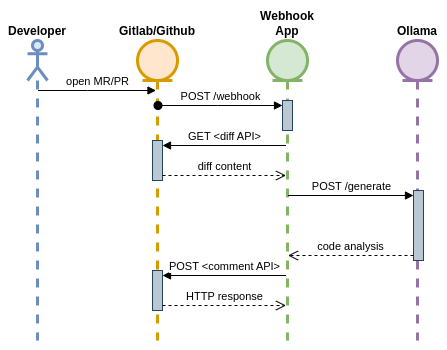
\includegraphics[width=0.7\textwidth]{sequence.png}
    \caption{Sequence Diagram}
    \label{fig:sequence}
\end{figure}

Check Figure~\ref{fig:systemdesign} and Figure~\ref{fig:sequence}  

\subsection{Implementation}
Mencionar o prompt e o modelo escolhidos pra enviar pro ollama
a organização dos diffs
constraints relacionados aos diffs

\subsection{Tests}
\begin{figure}[htbp]
    \centering
    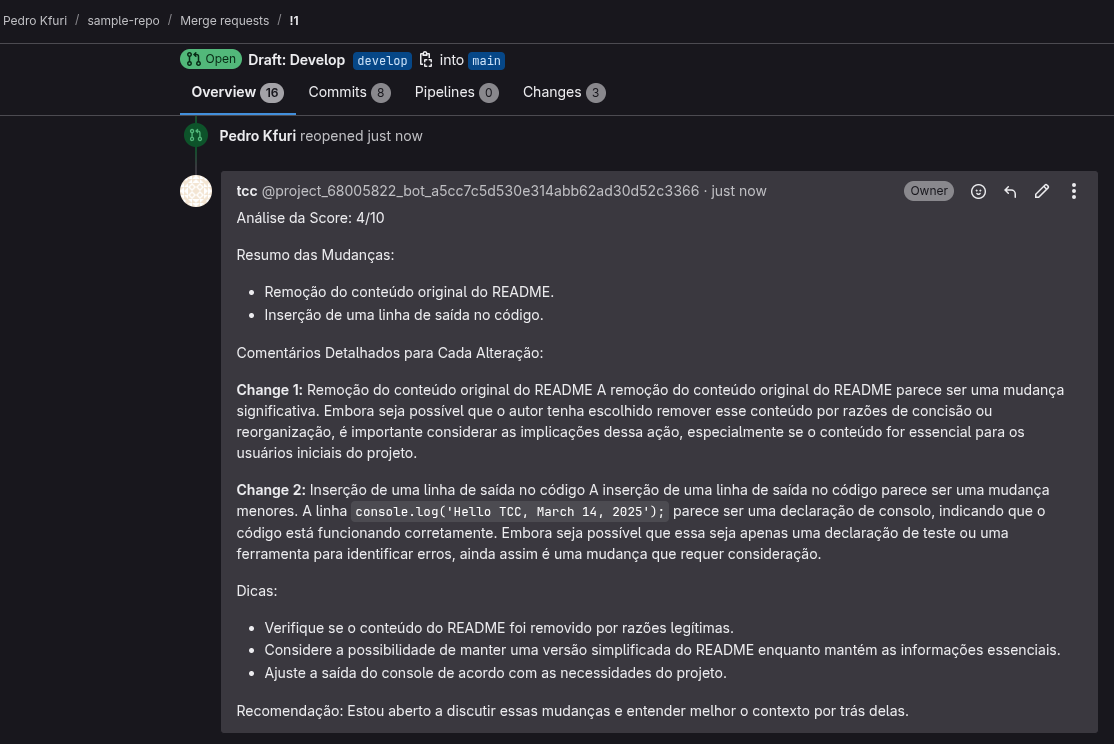
\includegraphics[width=1\textwidth]{gitlab.png}
    \caption{Gitlab comment generated}
    \label{fig:gitlab}
\end{figure}

\begin{figure}[htbp]
    \centering
    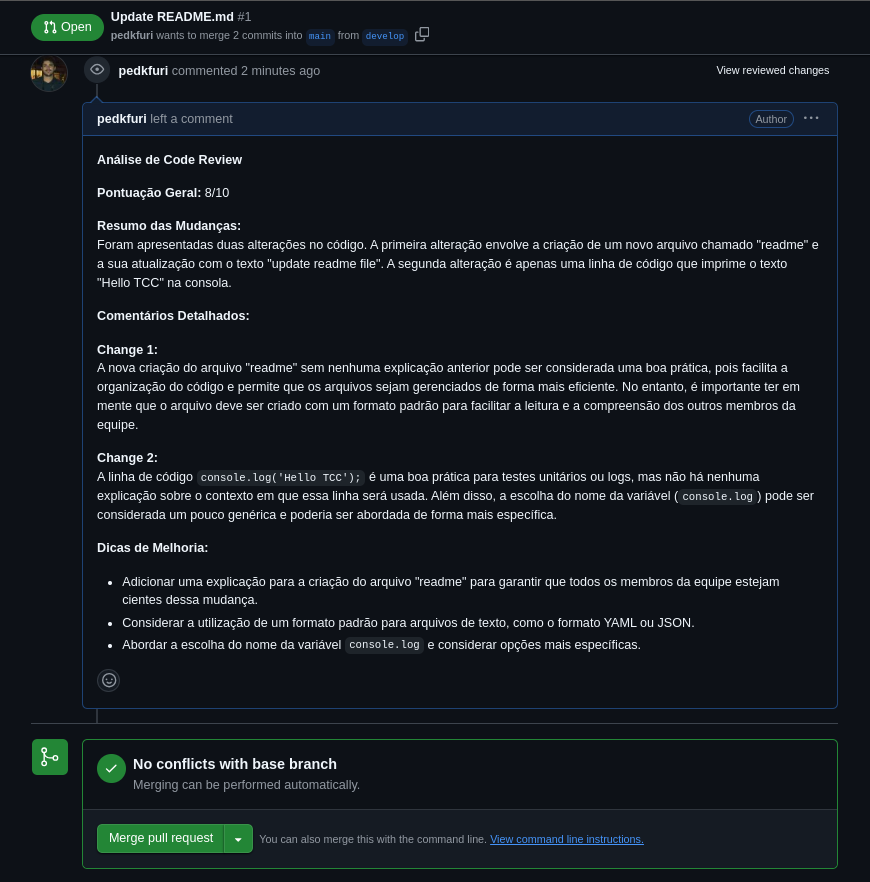
\includegraphics[width=1\textwidth]{github.png}
    \caption{Github comment generated}
    \label{fig:github}
\end{figure}

Check Figure~\ref{fig:gitlab} and Figure~\ref{fig:github} 

\section{Results}
Despite these benefits, challenges remain in integrating LLMs into DevOps workflows. AI models sometimes struggle with contextual understanding, leading to false positives or missed issues. Ensuring seamless integration with existing CI/CD pipelines requires robust API support and compatibility with established DevOps tools. Additionally, the quality of training data influences AI performance, highlighting the need for continuous refinement of machine learning models to reduce biases and improve decision-making. \cite{integratingAIDevops}
    
The future of AI-powered code review in DevOps lies in advancing context-aware models, improving explainability, and incorporating reinforcement learning for continuous improvement. Hybrid approaches that combine AI insights with human expertise may offer an optimal balance between automation and quality assurance. As AI continues to evolve, its role in DevOps will expand, offering organizations improved efficiency, reduced operational overhead, and enhanced software security and reliability. \cite{intelligentDevops}

\section{Conclusion}
Mencionar trabalhos futuros

\bibliographystyle{sbc}
\bibliography{references}
\end{document}
